\documentclass[a4paper,12pt]{article}
\usepackage[a4paper,top=1.3cm,bottom=2cm,left=1.5cm,right=1.5cm,marginparwidth=0.75cm]{geometry}
\usepackage{cmap}
\usepackage{mathtext}
\usepackage[T2A]{fontenc}
\usepackage[utf8]{inputenc}
\usepackage[english,russian]{babel}
\usepackage{siunitx}

\usepackage{graphicx}

\usepackage{wrapfig}
\usepackage{tabularx}
\usepackage{multirow}

\usepackage{hyperref}
\usepackage[rgb]{xcolor}
\hypersetup{
colorlinks=true,urlcolor=blue
}
\usepackage{amsmath,amsfonts,amssymb,amsthm,mathtools}
\usepackage{icomma}
\mathtoolsset{showonlyrefs=false}
\usepackage{euscript}
\usepackage{mathrsfs}
\DeclareMathOperator{\sgn}{\mathop{sgn}}
\newcommand*{\hm}[1]{#1\nobreak\discretionary{}
{\hbox{$\mathsurround=0pt #1$}}{}}

%%% Заголовок
\author{Макаров Лев Евгеньевич}
\title{Лабораторная работа №2.3.1

Определение Cp/Cv по скорости звука в газе
}
\date{\today}


\begin{document}

\begin{titlepage}
	\begin{center}
		{\large МОСКОВСКИЙ ФИЗИКО-ТЕХНИЧЕСКИЙ ИНСТИТУТ (НАЦИОНАЛЬНЫЙ ИССЛЕДОВАТЕЛЬСКИЙ УНИВЕРСИТЕТ)}
	\end{center}
	\begin{center}
		{\large Физтех-школа фотоники, электроники и молекулярной физики}
	\end{center}
	
	
	\vspace{4.5cm}
	{\huge
		\begin{center}
			{\bf Отчёт о выполнении лабораторной работы 2.1.3}\\
			Определение Cp/Cv по скорости звука в газе
		\end{center}
	}
	\vspace{2cm}
	\begin{flushright}
		{\LARGE Автор:\\ Макаров Лев Евгеньевич \\
			\vspace{0.2cm}
			Б04-306}
	\end{flushright}
	\vspace{8cm}
	\begin{center}
		Долгопрудный 2024
	\end{center}
\end{titlepage}

\section{Введение}

\textbf{Цель работы:} 
\begin{enumerate}
	\item измерение частоты колебаний и длины волны при резонансе звуковых колебаний в газе, заполняющем трубу
    \item определение показателя адиабаты с помощью уравнения состояния идеального газа
\end{enumerate}

\textbf{В работе используются:} 
\begin{itemize}
    \item звуковой генератор ГЗ
    \item электронный осциллограф ЭО
    \item микрофон
    \item телефон
    \item раздвижная труба
    \item теплоизолированная труба, обогреваемая водой из термостата
    \item баллон со сжатым углекислым газом
    \item газгольдер
\end{itemize}
\medskip

\section{Теоретические сведения}

Скорость распространения звуковой волны в газах зависит от показателя адиабаты $\gamma$. На измерении скорости звука основан один из наиболее точных методов определения показателя адиабаты. Скорость звука в газах определяется формулой:

\begin{equation*}
    c = \sqrt{\gamma \frac{RT}{\mu}}
\end{equation*}

Отсюда можно выразить показатель адиабаты:

\begin{equation}\label{1}
    \gamma = \frac{\mu}{RT} c^2
\end{equation}

Таким образом, для определения показателя адиабаты достаточно измерить температуру газа и скорость звука.

Звуковая волна, распространяющаяся вдоль трубы, испытывает многократные отражения от торцов. Звуковые колебания в трубе являются наложением всех отраженных волн и, вообще говоря, очень сложны. Картина упрощается, если длина трубы $L$ равна целому числу полуволн, то есть когда

\begin{equation}\label{2}
    L = n \lambda / 2
\end{equation}

Если это условие выполнено, то в трубе наступает резонанс.

Скорость звука c связана с его частотой $f$ и длиной волны $\lambda$ соотношением

\begin{equation}\label{3}
    c = \lambda f
\end{equation}

Подбор условий, при которых возникает резонанс, можно производить двояко:

\begin{enumerate}
    \item При неизменной частоте $f$ звукового генератора (а следовательно, и неизменной длине звуковой волны $\lambda$) можно изменять длину трубы $L$. Для этого применяется раздвижная труба. Длина раздвижной трубы постепенно увеличивается, и наблюдается ряд последовательных резонансов. Возникновение резонанса легко наблюдать на осциллографе по резкому увеличению амплитуды колебаний. Для последовательных резонансов имеем
    
    \begin{equation*}
        L_n = n \frac{\lambda}{2}, \ \ L_{n + 1} = (n + 1) \frac{\lambda}{2}, \ \ . . ., \ \ L_{n + k} = n \frac{\lambda}{2} + k \frac{\lambda}{2} 
    \end{equation*}
    
    т. е. $\lambda/2$ равно угловому коэффициенту графика, изображающего зависимость длины трубы $L$ от номера резонанса $k$. Скорость звука находится по формуле \eqref{3}.
    \item При постоянной длине трубы можно изменять частоту звуковых колебаний. В этом случае следует плавно изменять частоту $f$ звукового генератора, а следовательно, и длину звуковой волны $\lambda$. Для последовательных резонансов получим

    \begin{equation}\label{4}
        L = \frac{\lambda_1}{2}n = \frac{\lambda_2}{2}(n + 1) = ... = \frac{\lambda_{k + 1}}{2} (n + k)
    \end{equation}

    Из \eqref{3} и \eqref{4} имеем

    \begin{equation*}
        f_1 = \frac{c}{\lambda_1} = \frac{c}{2L}n, \ \ \ f_2 = \frac{c}{\lambda_2} = \frac{c}{2L}(n + 1) = f_1 + \frac{c}{2L}, ..., 
    \end{equation*}

    \begin{equation}\label{5}
        f_{k + 1} = \frac{c}{\lambda_{k+1}} = \frac{c}{2L}(n + k) = f_1 + \frac{c}{2L}k
    \end{equation}

    Скорость звука, деленная на $2L$, определяется, таким образом, по угловому коэффициенту графика зависимости частоты от номера резонанса.
\end{enumerate}

\section{Оборудование и экспериментальные погрешности}

Соответственно двум методам измерения скорости звука в работе имеются две установки (рис. \ref{img:ustan-1} и \ref{img:ustan-2}). В обеих установках звуковые колебания в трубе возбуждаются телефоном Т и улавливаются микрофоном М. Мембрана телефона приводится в движение переменным током звуковой частоты; в качестве источника переменной ЭДС используется звуковой генератор ГЗ. Возникающий в микрофоне сигнал наблюдается на осциллографе ЭО. Микрофон и телефон присоединены к установке через тонкие резиновые трубки. Такая связь достаточна для возбуждения и обнаружения звуковых колебаний в трубе и в то же время мало возмущает эти колебания: при расчетах оба торца трубы можно считать неподвижными, а влиянием соединительных отверстий пренебречь. Первая установка (рис. \ref{img:ustan-1}) содержит раздвижную трубу с миллиметровой шкалой. Через патрубок (на рисунке не показан) труба может наполняться воздухом или углекислым газом из газгольдера. На этой установке производятся измерения $\gamma$ для воздуха и для CO2. Вторая установка (рис. \ref{img:ustan-2}) содержит теплоизолированную трубу постоянной длины. Воздух в трубе нагревается водой из термостата. Температура газа принимается равной температуре омывающей трубу воды. На этой установке измеряется зависимость скорости звука от температуры.

\begin{figure}[!h]
    \centering
    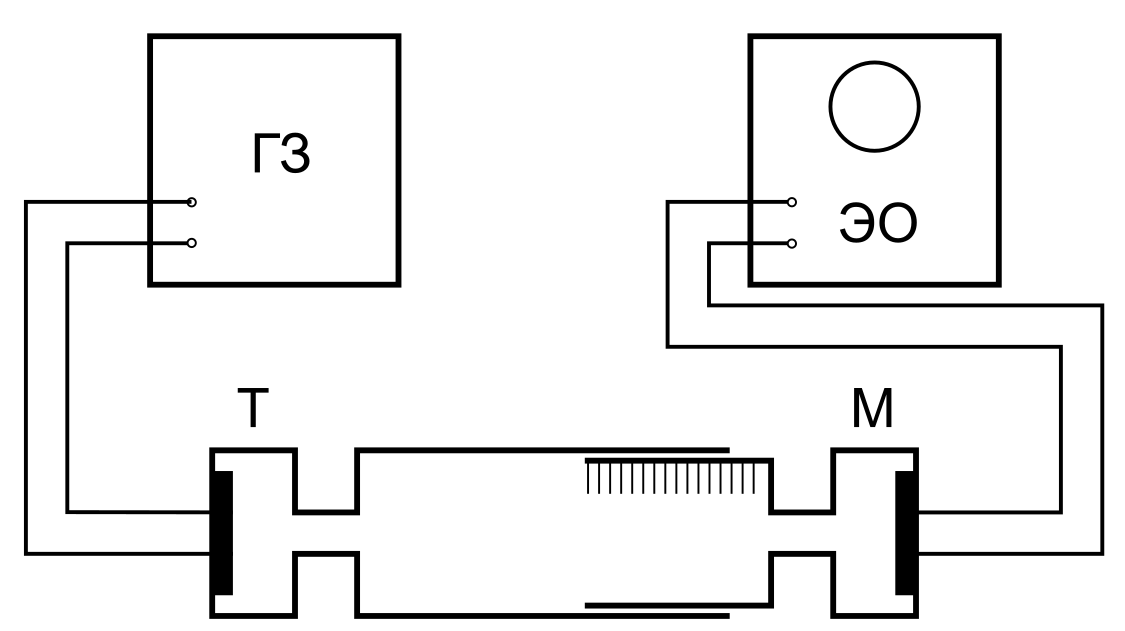
\includegraphics[width=9.5 cm]{ustan-1.png}
    \caption{Установка для измерения скорости звука при помощи раздвижной трубы}
    \label{img:ustan-1}
\end{figure}

\begin{figure}[!h]
    \centering
    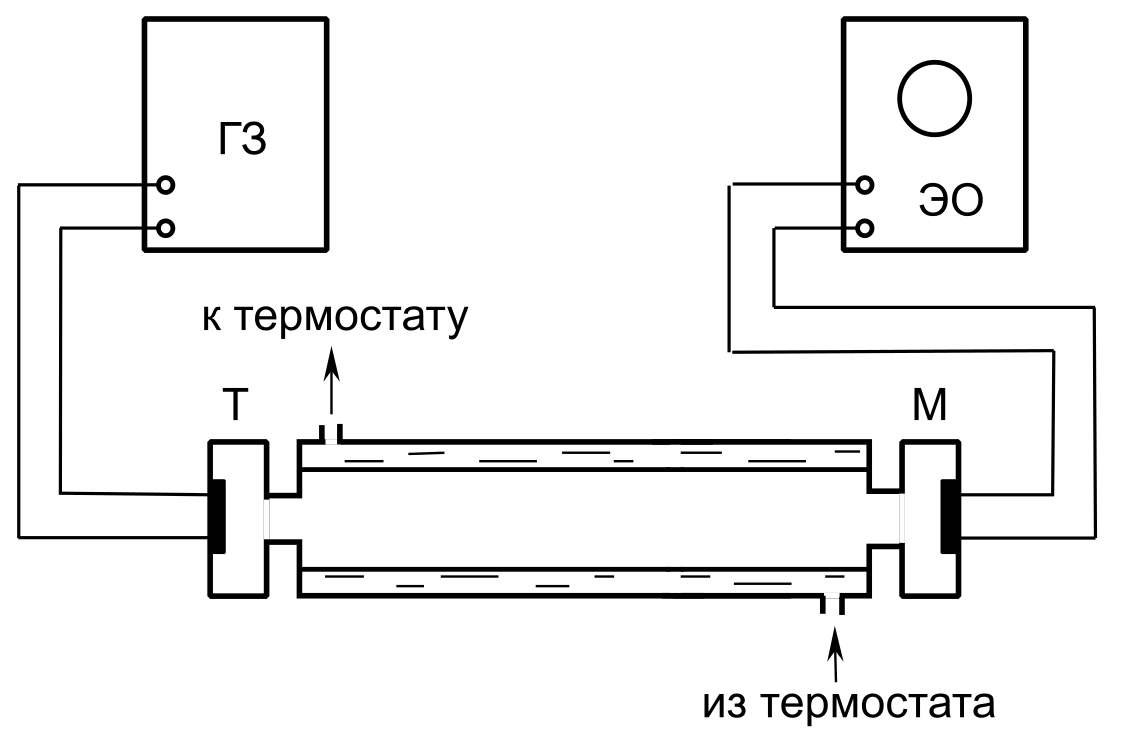
\includegraphics[width=9.5 cm]{ustan-2.png}
    \caption{Установка для изучения зависимости скорости звука от температуры}
    \label{img:ustan-2}
\end{figure}

\clearpage

\section{Результаты измерений и обработка данных}

\subsection{Подготовка приборов}

Включим в сеть электронный осциллограф и звуковой генератор, дадим им прогреться 5 минут. Настроим осциллограф так, чтобы на экране было видно линию, прочерченную электронным лучом.

На генераторе звука установим нулевое значение частоты.

\subsection{Подборка напряжения}

На выходе генератора такое напряжение, чтобы на экране осциллографа амплитуда колебаний была достаточной для определения резонанса.

\subsection{Измерения на первой установке}

Длина трубы в установке: $L = (740 \pm 1) $ мм

Постепенно увеличивая частоту на генераторе найдём значение частоты первого резонанса, полученною частоту запишем в таблицу \ref{table:resonance-1}

Далее по этой частоте можно приблизительно оценить значения следующих резонансных частот. Найдём значения резонансных частот, которые возможно определить осциллографом и запишем в таблицу \ref{table:resonance-1}.

Далее включим термостат (нужно также записать температуру в трубе) и проведём аналогичные измерения для температур: 35, 45 и 60 $C^\circ$. Результаты измерений запишем в таблицу \ref{table:resonance-1}.

\begin{table}[!ht]
    \centering
    \begin{tabular}{|l|l|l|l|l|}
    \hline
        $T$, К & 290,7 & 308,2 & 318,2 & 333,2 \\ \hline
        $T$, $C^\circ$ & 17,5 & 35 & 45 & 60 \\ \hline
        $n$ & $f$, Гц & $f$, Гц & $f$, Гц & $f$, Гц \\ \hline
        1 & 236 & 242 & 246 & 250 \\ \hline
        2 & 466 & 476 & 484 & 495 \\ \hline
        3 & 699 & 714 & 724 & 740 \\ \hline
        4 & 928 & 948 & 962 & 985 \\ \hline
        5 & 1158 & 1184 & 1202 & 1230 \\ \hline
        6 & 1390 & 1420 & 1442 & 1476 \\ \hline
        7 & 1620 & 1655 & 1682 & 1721 \\ \hline
        8 & 1852 & 1892 & 1922 & 1966 \\ \hline
        9 & 2083 & 2128 & 2161 & 2211 \\ \hline
        10 & 2313 & 2363 & 2400 & 2456 \\ \hline
        11 & 2544 & 2599 & ~ & ~ \\ \hline
        12 & 2774 & 2834 & ~ & ~ \\ \hline
        13 & 3005 & 3070 & ~ & ~ \\ \hline
        14 & 3236 & 3305 & ~ & ~ \\ \hline
    \end{tabular}\caption{\textit{Значения резонансов для четырёх температур}}\label{table:resonance-1}
\end{table}

Так как зависимость частоты от номера резонанса должна быть линейной, то для проверки зависимости можно воспользоваться МНК, для аппроксимации наилучшей прямой, где $x = k$, где $k = n - 1$, а $y = f$.

\begin{equation}\label{eq:mnk}
    k = \frac{\langle xy\rangle - \langle x \rangle \langle y \rangle}{\langle x^2 \rangle - \langle x \rangle^2},
    \ \text{а} \ \  b = \langle y \rangle - k\langle x \rangle
\end{equation}

Погрешности для $k$ и $b$ рассчитываются по формулам:

\begin{equation}
    \sigma_k = \frac{1}{\sqrt{n}} \sqrt{\frac{\langle y^2 \rangle - \langle y \rangle^2}{\langle x^2 \rangle - \langle x \rangle^2} - k^2}
\end{equation}

\begin{equation}
    \sigma_b = \sigma_k\sqrt{\langle x^2 \rangle - \langle x \rangle^2}
\end{equation}

Посчитаем все промежуточные значения и вычислим коэффициенты прямой.

\begin{equation*}
    k_1 = \frac{15034 - 6,5 \cdot 1736}{58,5 - {6,5}^2} \approx 230,77 \ \text{Гц}
\end{equation*}
\begin{equation*}
    \sigma_{k1} = \frac{1}{\sqrt{13}} \sqrt{\frac{3879114 - {1736}^2}{58,5 - {6,5}^2} - {230,77}^2} \approx 0,04 \ \text{Гц}
\end{equation*}



\begin{equation*}
    k_2 = \frac{15358 - 6,5 \cdot 1773}{58,5 - {6,5}^2} \approx 235,71 \ \text{Гц}
\end{equation*}
\begin{equation*}
    \sigma_{k2} = \frac{1}{\sqrt{13}} \sqrt{\frac{4048358 - {1773}^2}{58,5 - {6,5}^2} - {235,71}^2} \approx 0,04 \ \text{Гц}
\end{equation*}



\begin{equation*}
    k_3 = \frac{7927 - 4,5 \cdot 1322}{28,5 - {4,5}^2} \approx 239,48 \ \text{Гц}
\end{equation*}
\begin{equation*}
    \sigma_{k3} = \frac{1}{\sqrt{9}} \sqrt{\frac{2222168 - {1322}^2}{28,5 - {3,5}^2} - {239,48}^2} \approx 0,08 \ \text{Гц}
\end{equation*}



\begin{equation*}
    k_4 = \frac{8111 - 4,5 \cdot 1353}{28,5 - {4,5}^2} \approx 245,15 \ \text{Гц}
\end{equation*}
\begin{equation*}
    \sigma_{k4} = \frac{1}{\sqrt{9}} \sqrt{\frac{2326428 - {1353}^2}{28,5 - {3,5}^2} - {245,15}^2} \approx 0,03 \ \text{Гц}
\end{equation*}

Все прямые и экспериментальные точки изобразим на рисунке \ref{pic:graph-1}.

Согласно формуле \eqref{5} свободными членами являются значения первого резонанса. Из этой формулы следует:

\begin{equation}\label{eq:c}
    c_i = 2 L k_i
\end{equation}

Для каждой серии измерений посчитаем скорость звука и запишем в таблицу \ref{table:res-1}.

Погрешность измерения скорости звука вычисляется по формуле:

\begin{equation}\label{eq:sigma-c}
    \sigma_c = c \sqrt{\left( \frac{\sigma_k}{k} \right)^2 + \left( \frac{\sigma_L}{L} \right)^2}
\end{equation}

Посчитаем их и запишем в таблицу \ref{table:res-1}.

\begin{table}[!ht]
    \centering
    \begin{tabular}{|l|l|l|l|l|}
    \hline
        $T$, $C^\circ$ & 17,5 & 35 & 45 & 60 \\ \hline
        $c$, м/с & 341,5 & 348,8 & 354,4 & 362,8 \\ \hline
        $\sigma_c$, м/с & 0,5 & 0,5 & 0,5 & 0,5 \\ \hline
        $\gamma$ & 1,401 & 1,378 & 1,378 & 1,379 \\ \hline
        $\sigma_\gamma$ & 0,004 & 0,004 & 0,004 & 0,004 \\ \hline
    \end{tabular}\caption{\textit{Вычисление скорости звука для четырёх температур}}\label{table:res-1}
\end{table}

По формуле \eqref{1} вычислим показатель адиабаты $\gamma$ для каждой температуры и запишем в таблицу \ref{table:res-1}. 

Погрешность измерения $\gamma$ можно вычислить по формуле:

\begin{equation}\label{eq:sigma-gamma}
    \sigma_\gamma = \sqrt{
    \left( \frac{\gamma}{T} \right)^2 \sigma_T^2 + 
    \left( \frac{2\gamma}{c} \right)^2 \sigma_c^2
    } = \gamma \sqrt{\left( \frac{\sigma_T}{T} \right)^2 + \left( \frac{2 \sigma_c}{c} \right)^2}
\end{equation}

Вычислим погрешность и запишем её в таблицу \ref{table:res-1}.

Тогда в качестве значения $\gamma$ возьмём среднее:

\begin{equation*}
    \gamma = 1,384 \pm 0,004
\end{equation*}

\subsection{Измерения на второй установке}

Длина трубки в данном опыте $L = (795 \pm 1)$ мм

Проведём аналогичные измерения для углекислого газа и одного значения температуры ($t_\text{к} = 24,4 \ C^\circ$). Измерения запишем в таблицу \ref{table:resonance-2}. В этой таблице сразу посчитаем промежуточные значения МНК.

\begin{table}[!ht]
    \centering
    \begin{tabular}{|l|l|l|l|l|l|}
    \hline
        ~ & n & f, Гц & x\^2  & y\^2  & x*y  \\ \hline
        ~ & 1 & 342 & 1 & 116964 & 342 \\ \hline
        ~ & 2 & 673 & 4 & 452929 & 1346 \\ \hline
        ~ & 3 & 1006 & 9 & 1012036 & 3018 \\ \hline
        ~ & 4 & 1339 & 16 & 1792921 & 5356 \\ \hline
        ~ & 5 & 1671 & 25 & 2792241 & 8355 \\ \hline
        ~ & 6 & 2005 & 36 & 4020025 & 12030 \\ \hline
        ~ & 7 & 2339 & 49 & 5470921 & 16373 \\ \hline
        ~ & 8 & 2677 & 64 & 7166329 & 21416 \\ \hline
        ~ & 9 & 3014 & 81 & 9084196 & 27126 \\ \hline
        ~ & 10 & 3349 & 100 & 11215801 & 33490 \\ \hline
        ср & 5,5 & 1841,5 & 38,5 & 4312436,3 & 12885,2 \\ \hline
    \end{tabular}\caption{\textit{Значение резонансов для углекислого газа}}\label{table:resonance-2}
\end{table}

Значения коэффициентов наилучшей прямой:

\begin{equation*}
    k_1 = \frac{12885,2 - 5,5 \cdot 1841,5}{38,5 - {5,5}^2} \approx 334,2 \ \text{Гц}
\end{equation*}
\begin{equation*}
    \sigma_{k1} = \frac{1}{\sqrt{10}} \sqrt{\frac{4312436,3 - {1841,5}^2}{38,5 - {5,5}^2} - {334,2}^2} \approx 0,3 \ \text{Гц}
\end{equation*}

Прямую и экспериментальные точки изобразим на рисунке \ref{pic:graph-2}.

Вычислим скорость звука и ее погрешность по формулам \eqref{eq:c} и \eqref{eq:sigma-c} соответственно:

\begin{equation*}
    c = (531,3 \pm 0,8) \ \text{м/с}
\end{equation*}

Далее по формулам \eqref{1} и \eqref{eq:sigma-gamma} вычислим $\gamma$ и ее погрешность:

\begin{equation*}
    \gamma = 5,02 \pm 0,02
\end{equation*}


\begin{figure}[h!]
        \centering
	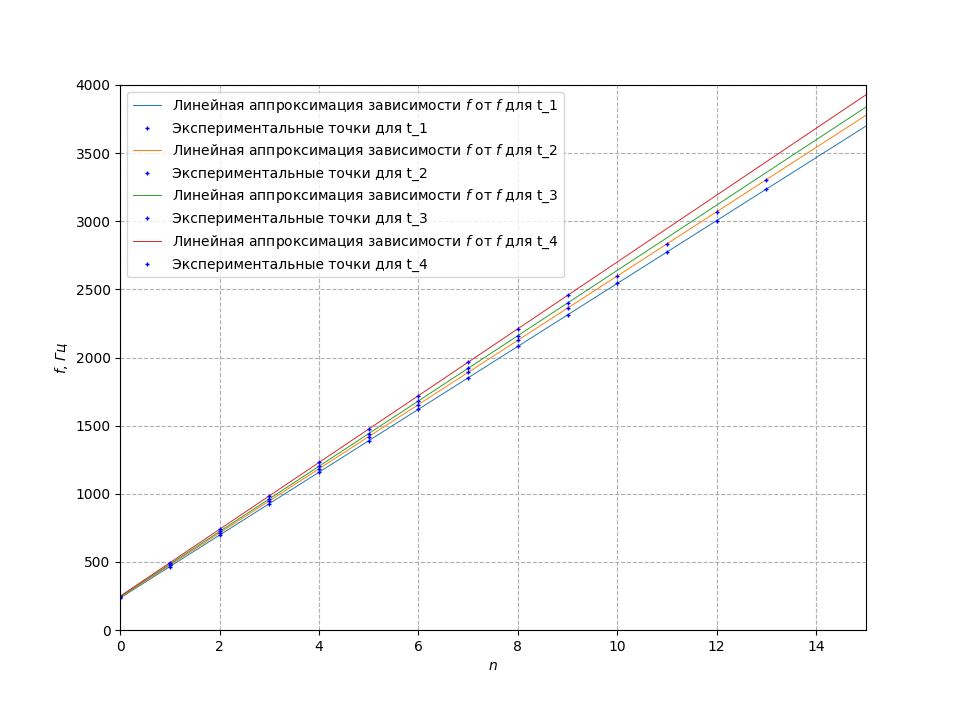
\includegraphics[width=1.1\textwidth]{graph-1.png}
	\caption{\textit{График зависимости $f$ от $k$ для первой установки}}
	\label{pic:graph-1}
\end{figure}

\begin{figure}[h!]
        \centering
	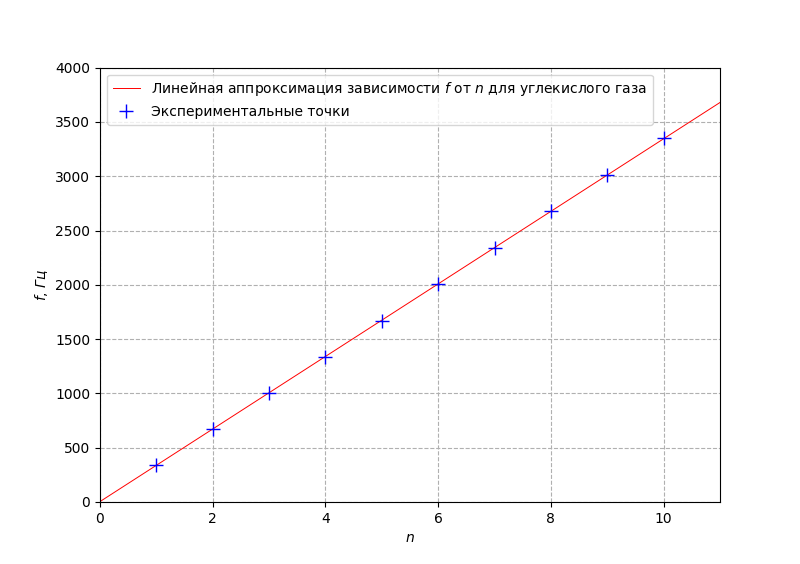
\includegraphics[width=1.1\textwidth]{graph-2.png}
	\caption{\textit{График зависимости $f$ от $k$ для второй установки}}
	\label{pic:graph-2}
\end{figure}

\end{document}